\documentclass[11pt,a4paper]{article}
\usepackage[utf8]{inputenc}
\usepackage[spanish,es-tabla]{babel}
\usepackage{geometry}
\geometry{top=3cm, bottom=3cm, left=2.5cm, right=2.5cm}
\usepackage{amsmath}
\usepackage{amsfonts}
\usepackage{amssymb}
\usepackage{graphicx}
\usepackage{booktabs}
\usepackage{array}
\usepackage{listings}
\usepackage{xcolor}
\usepackage{hyperref}
\usepackage{fancyhdr}
\usepackage{titlesec}
\usepackage{microtype}
\usepackage{lmodern}
\usepackage{longtable}
\usepackage{tabularx}
\usepackage{multirow}
\usepackage{enumitem}
\usepackage{tcolorbox}
\tcbuselibrary{skins, breakable}
\usepackage{float}

% ── Colores formales ─────────────────────────────────────────────────────────
\definecolor{navy}{RGB}{26, 54, 93}
\definecolor{darkgray}{RGB}{60, 60, 60}
\definecolor{codebg}{RGB}{245, 247, 250}
\definecolor{codeborder}{RGB}{220, 225, 230}
\definecolor{citegreen}{RGB}{40, 120, 40}
\definecolor{warnorange}{RGB}{180, 80, 0}
\definecolor{okgreen}{RGB}{20, 110, 50}
\definecolor{alertred}{RGB}{160, 20, 20}

% ── Cajas coloreadas ─────────────────────────────────────────────────────────
\newtcolorbox{infobox}[1][]{colback=codebg, colframe=navy!60, fonttitle=\bfseries\sffamily, title=#1, breakable}
\newtcolorbox{warnbox}[1][]{colback=yellow!8, colframe=warnorange, fonttitle=\bfseries\sffamily, title=#1, breakable}
\newtcolorbox{okbox}[1][]{colback=green!5, colframe=okgreen, fonttitle=\bfseries\sffamily, title=#1, breakable}

% ── Hipervínculos ─────────────────────────────────────────────────────────────
\hypersetup{
    colorlinks=true, linkcolor=navy, filecolor=magenta,
    urlcolor=navy, citecolor=citegreen,
    pdftitle={Proyecto 3 - Sistemas Distribuidos Tolerantes a Fallos},
    pdfpagemode=FullScreen,
}

% ── Cabecera y pie de página ──────────────────────────────────────────────────
\pagestyle{fancy}
\fancyhf{}
\renewcommand{\headrulewidth}{0.4pt}
\renewcommand{\footrulewidth}{0.4pt}
\lhead{\textcolor{navy}{\small\sffamily Proyecto 3 — Sistemas Distribuidos}}
\rhead{\textcolor{darkgray}{\small\sffamily Salud Digital · Universidad de Talca}}
\lfoot{\textcolor{darkgray}{\scriptsize\sffamily Hernandez · Muñoz · Martinez · Paredes}}
\rfoot{\textcolor{navy}{\small\sffamily Página \thepage}}

% ── Secciones ─────────────────────────────────────────────────────────────────
\titleformat{\section}
  {\normalfont\Large\bfseries\color{navy}}
  {\thesection}{1em}{}[{\color{navy}\titlerule[0.8pt]}]
\titleformat{\subsection}
  {\normalfont\large\bfseries\color{navy!85}}
  {\thesubsection}{1em}{}
\titleformat{\subsubsection}
  {\normalfont\normalsize\bfseries\color{darkgray}}
  {\thesubsubsection}{1em}{}

% ── Código fuente ─────────────────────────────────────────────────────────────
\lstset{
    backgroundcolor=\color{codebg},
    basicstyle=\ttfamily\small\color{darkgray},
    breakatwhitespace=false, breaklines=true, captionpos=b,
    commentstyle=\color{gray},
    keepspaces=true,
    keywordstyle=\color{navy}\bfseries,
    numbers=left, numberstyle=\tiny\color{gray!80}, numbersep=8pt,
    showspaces=false, showstringspaces=false, showtabs=false,
    tabsize=2, stringstyle=\color{purple},
    frame=single, rulecolor=\color{codeborder}, frameround=tttt
}

% ── Comandos de estado ────────────────────────────────────────────────────────
\newcommand{\ok}{\textcolor{okgreen}{\textbf{✓}}}
\newcommand{\warn}{\textcolor{warnorange}{\textbf{⚠}}}
\newcommand{\fail}{\textcolor{alertred}{\textbf{✗}}}

% =============================================================================
\begin{document}

% ─────────────────────────────────────────────────────────────────────────────
%  PORTADA
% ─────────────────────────────────────────────────────────────────────────────
\begin{titlepage}
    \centering
    \vspace*{1.5cm}
    {\scshape\Large Universidad de Talca \par}
    {\scshape\large Facultad de Ingeniería y Ciencias Aplicadas \par}
    \vspace{0.4cm}
    {\large Sistemas Operativos y Distribuidos \par}
    \vspace{1.5cm}
    {\huge\bfseries\color{navy}
        Infraestructura Distribuida y Tolerante a Fallos\\[0.4cm]
        para Entornos de Salud Digital \par}
    \vspace{0.8cm}
    {\large\textcolor{darkgray}{
        Sistema clínico multi-VM con replicación de datos, failover automático,
        middleware de contingencia y módulo de bodega integrado} \par}
    \vspace{2.5cm}

    \begin{tabular}{p{4cm}l}
        \textbf{Integrantes:} & Krisstal Hernandez \\
                              & Mariano Muñoz \\
                              & Felipe Martinez \\
                              & Maximiliano Paredes \\[0.3cm]
        \textbf{Docente:}     & rpavez@utalca.cl \\[0.2cm]
        \textbf{Fecha:}       & 7 de julio de 2026 \\[0.2cm]
        \textbf{Entrega:}     & 2 (Final) — Proyecto Unidad 3
    \end{tabular}

    \vfill
    \begin{center}
        \small\sffamily\color{darkgray}
        Proyecto 3: Sistemas Distribuidos\\
        Tolerancia a Fallos en Infraestructura de Centro de Salud Regional
    \end{center}
\end{titlepage}

\newpage
\tableofcontents
\newpage

% =============================================================================
\section{Introducción y Contexto}
% =============================================================================

\subsection{Contexto del problema}

Un centro de salud de referencia regional requiere modernizar su infraestructura tecnológica,
migrando desde un modelo 100\% local hacia un procesamiento distribuido en datos y cómputo.
La manipulación de fichas clínicas es una responsabilidad crítica, con exigencia legal de
persistencia de datos por al menos 5 años, lo que hace indispensable garantizar la continuidad
operacional incluso ante fallos de red, servidores o bases de datos.

Este proyecto implementa una arquitectura distribuida y tolerante a fallos que simula el
ecosistema tecnológico del centro de salud, cubriendo los módulos de Estaciones Médicas,
Terminales Administrativas, Middleware de integración y Sistema de Bodega e Inventario.

\subsection{Objetivos}

\begin{itemize}[leftmargin=1.5em]
    \item Diseñar e implementar una topología distribuida en 3 máquinas virtuales en Google
          Cloud Platform, con redes segmentadas (\texttt{hospital\_net}, \texttt{cloud\_net},
          \texttt{dmz\_net}).
    \item Garantizar la tolerancia a fallos en las capas de aplicación, base de datos e
          integración mediante réplicas, orquestadores y colas de contingencia.
    \item Incorporar un módulo adicional (Sistema de Bodega) que se integre al flujo clínico
          de forma transparente.
    \item Documentar los Acuerdos de Nivel de Servicio (SLA) y Objetivos de Nivel de Servicio
          (SLO) del sistema.
    \item Validar el sistema mediante las tres pruebas de tolerancia a fallos requeridas.
\end{itemize}

% =============================================================================
\section{Arquitectura General y Topología de Red}
% =============================================================================

\subsection{Visión general — 3 Máquinas Virtuales en GCP}

El sistema se despliega sobre tres Máquinas Virtuales (VMs) en la zona
\texttt{us-central1-a} de Google Cloud Platform, interconectadas mediante una VPC privada:

\begin{center}
\begin{tabular}{llll}
\toprule
\textbf{VM} & \textbf{Nombre} & \textbf{IP Privada} & \textbf{Rol Principal} \\
\midrule
VM 1 & vm-hospital-local   & 10.128.0.10 & Estaciones Médicas + MariaDB \\
VM 2 & vm-nube-central     & 10.128.0.20 & Terminales Administrativas + PostgreSQL \\
VM 3 & vm-gateway          & 10.128.0.30 & Nginx Gateway + Middleware + Bodega + MySQL \\
\bottomrule
\end{tabular}
\end{center}

\begin{lstlisting}[language=bash, caption=Topología lógica del sistema distribuido]
         [ Navegador del Usuario / Cliente ]
                         |
              ( HTTPS / WSS -- Cloudflare )
                         |
              [ VM3: Cloudflare Tunnel ]
                         | (Tunel Inverso Seguro)
              [ VM3: Nginx Proxy Inverso ]
         ________________|_______________
        |                               |
   /ws-medicas                  /ws-administrativas
        |                               |
[ VM1: Hospital Local ]      [ VM2: Nube Central ]
  app-estaciones (8001)        app-terminales (8002)
  app-estaciones-replica       app-terminales-replica
  HAProxy MariaDB (3306)       HAProxy PostgreSQL (5432)
  MariaDB Master               PostgreSQL Master
  MariaDB Replica              PostgreSQL Replica
        |                               |
        |___________ HTTP POST _________|
                         |
              [ VM3: Middleware (8000) ]
                  SQLite contingencia
                         |
              [ VM3: App Bodega (8003) ]
              HAProxy MySQL (3306)
              MySQL Master + Replica
\end{lstlisting}

\subsection{Heterogeneidad tecnológica}

El enunciado requiere que las aplicaciones 1 y 2 estén desarrolladas en lenguajes distintos.
Esta restricción fue implementada de la siguiente forma:

\begin{table}[h!]
\centering
\begin{tabular}{lllll}
\toprule
\textbf{Módulo} & \textbf{Lenguaje} & \textbf{Framework} & \textbf{Base de Datos} & \textbf{Puerto} \\
\midrule
App 1 — Estaciones Médicas   & Node.js 18 & Socket.io + mysql2   & MariaDB 10.11   & 8001 \\
App 2 — Terminales Admin.    & Python 3.10 & python-socketio + asyncpg & PostgreSQL 16 & 8002 \\
App 3 — Bodega               & Node.js 18 & Express + mysql2    & MySQL 8.0       & 8003 \\
Middleware                   & Node.js 18 & Express + SQLite    & MySQL 8.0       & 8000 \\
\bottomrule
\end{tabular}
\caption{Stack tecnológico por módulo de aplicación.}
\end{table}

\subsection{Segmentación de redes}

\begin{itemize}
    \item \textbf{\texttt{hospital\_net}:} Red interna del hospital. Conecta la VM1 con la VM3.
          Permite la operación local de las estaciones médicas sin depender de Internet.
    \item \textbf{\texttt{cloud\_net}:} Red de la nube. Conecta la VM2 con la VM3.
          Consolida las admisiones administrativas en un repositorio central.
    \item \textbf{\texttt{dmz\_net}:} Zona desmilitarizada. Solo Nginx y Cloudflare Tunnel
          tienen presencia aquí, aislando los servicios internos del tráfico externo.
\end{itemize}

% =============================================================================
\section{Componentes del Sistema}
% =============================================================================

\subsection{App 1 — Estaciones Médicas (Node.js / MariaDB)}

El servidor levanta un WebSocket en el puerto 8001 bajo el path \texttt{/ws-medicas},
reconocible por el proxy Nginx. La aplicación se conecta a MariaDB a través del
proxy HAProxy local (\texttt{db-local-proxy:3306}), de modo que nunca conoce
la dirección real del nodo maestro o réplica.

Eventos implementados:
\begin{itemize}
    \item \textbf{\texttt{consultar\_paciente}:} Búsqueda por RUT en la tabla
          \texttt{fichas\_pacientes} de MariaDB.
    \item \textbf{\texttt{actualizar\_diagnostico}:} Actualiza el campo
          \texttt{diagnostico} y notifica de forma asíncrona al Middleware.
\end{itemize}

\subsection{App 2 — Terminales Administrativas (Python / PostgreSQL)}

Desarrollado en Python 3.10 con \texttt{aiohttp} + \texttt{python-socketio}, levanta
el servicio en el puerto 8002 bajo el path \texttt{/ws-administrativas}.
Utiliza \texttt{asyncpg} para conexiones asíncronas de alta eficiencia a PostgreSQL
a través del proxy HAProxy (\texttt{db-nube-proxy:5432}).

Implementa Control de Acceso Basado en Roles (RBAC): solo usuarios con
\texttt{rol = "administrativo"} pueden ejecutar el evento \texttt{admitir\_paciente},
rechazando intentos de otros roles con un mensaje de error explícito.

\subsection{App 3 — Sistema de Bodega (Node.js / MySQL)}

Módulo adicional que representa el Sistema de Bodega e Inventario del centro de salud.
Expone una API REST en el puerto 8003:

\begin{itemize}
    \item \textbf{\texttt{GET /api/inventario}:} Retorna el stock actual de todos los insumos.
    \item \textbf{\texttt{POST /api/inventario/descontar}:} Descuenta unidades de un insumo
          dado su código y cantidad, con validación de stock mínimo.
\end{itemize}

El Middleware activa automáticamente el descuento al detectar palabras clave en el
texto del diagnóstico médico (ej. ``Paracetamol 500mg'', ``Ibuprofeno 600mg'', ``Enalapril 10mg'').

\subsection{Middleware — API Gateway y Cola de Contingencia}

El Middleware (Node.js/Express, puerto 8000) actúa como broker central entre las
aplicaciones y la base de datos MySQL central. Sus responsabilidades son:

\begin{enumerate}
    \item \textbf{Enrutamiento:} Recibe notificaciones HTTP POST de App 1 y App 2 y
          las persiste en MySQL central.
    \item \textbf{Análisis de recetas:} Detecta medicamentos en los diagnósticos y
          solicita el descuento a la App de Bodega.
    \item \textbf{Cola de contingencia SQLite:} Si MySQL o la App de Bodega están
          caídas, guarda la transacción en una base SQLite local
          (\texttt{contingencia.db}) y la sincroniza automáticamente cuando el
          servicio vuelve a estar en línea (worker cada 10 segundos).
\end{enumerate}

\begin{lstlisting}[language=JavaScript, caption=Worker de sincronización de contingencia (middleware/server.js)]
// Tipos de operaciones encoladas
// ADMITIR_PACIENTE  -- desde App 2 cuando la DB central falla
// GUARDAR_DIAGNOSTICO -- desde App 1 cuando la DB central falla
// DESCONTAR_BODEGA  -- cuando la App 3 no responde

setInterval(procesarColaContingencia, 10000); // cada 10 segundos

async function procesarColaContingencia() {
    // Obtiene hasta 5 elementos pendientes ordenados cronologicamente
    contingenciaDb.all(
        'SELECT * FROM cola_contingencia ORDER BY id ASC LIMIT 5',
        async (err, rows) => {
            // Intenta reconectar a MySQL Central
            connection = await mysql.createConnection(mysqlConfig);
            for (const row of rows) {
                // Procesa segun tipo y elimina si fue exitoso
                contingenciaDb.run(
                    'DELETE FROM cola_contingencia WHERE id = ?', [row.id]
                );
            }
        }
    );
}
\end{lstlisting}

% =============================================================================
\section{Tolerancia a Fallos — Alta Disponibilidad}
% =============================================================================

\subsection{Capa de Aplicación — Nginx con failover}

Nginx (VM3) actúa como proxy inverso y balanceador de carga. Se configura un bloque
\texttt{upstream} con política de backup:

\begin{lstlisting}[language=bash, caption=Configuración de upstream con failover en Nginx]
upstream ws_medicas {
    server 10.128.0.10:8001 max_fails=1 fail_timeout=5s;
    server 10.128.0.10:8011 backup;  # replica de app-estaciones
}

upstream ws_administrativas {
    server 10.128.0.20:8002 max_fails=1 fail_timeout=5s;
    server 10.128.0.20:8012 backup;  # replica de app-terminales
}
\end{lstlisting}

Si la aplicación principal falla, Nginx detecta el fallo tras 1 reintento y redirige
el tráfico a la réplica en menos de 5 segundos, de forma transparente para el usuario.

\subsection{Capa de Base de Datos — HAProxy con health checks}

Cada VM ejecuta un proxy TCP (HAProxy 2.8) que realiza health checks cada 3 segundos.
Las aplicaciones nunca se conectan directamente a una instancia de base de datos;
siempre acceden a través del proxy:

\begin{table}[h!]
\centering
\begin{tabular}{llll}
\toprule
\textbf{VM} & \textbf{Proxy} & \textbf{BD Primaria} & \textbf{BD Réplica (backup)} \\
\midrule
VM 1 & db-local-proxy:3306  & db-local-master  & db-local-replica  \\
VM 2 & db-nube-proxy:5432   & db-nube-master   & db-nube-replica   \\
VM 3 & db-central-proxy:3306 & db-central-master & db-central-replica \\
\bottomrule
\end{tabular}
\caption{Orquestadores de base de datos por VM.}
\end{table}

\subsection{Capa de Integración — Cola de contingencia SQLite}

Si el Middleware no puede escribir en MySQL o contactar a la App de Bodega,
guarda la operación en \texttt{cola\_contingencia} (SQLite) con estado PENDING.
Un worker en segundo plano reintenta cada 10 segundos hasta que el servicio
vuelve a estar disponible, procesando las operaciones en orden cronológico (FIFO).

% =============================================================================
\section{Distribución de Base de Datos}
% =============================================================================

Las bases de datos están distribuidas entre los tres servidores, cada una con su
propio dominio de datos y réplica local:

\begin{table}[h!]
\centering
\begin{tabularx}{\textwidth}{lXll}
\toprule
\textbf{Servidor} & \textbf{Datos almacenados} & \textbf{Motor} & \textbf{Replicación} \\
\midrule
VM 1 (10.128.0.10) & Fichas clínicas locales (\texttt{fichas\_pacientes}) & MariaDB 10.11 & Binlog ROW (lógica) \\
VM 2 (10.128.0.20) & Admisiones administrativas (\texttt{fichas\_pacientes}) & PostgreSQL 16 & pg\_basebackup (física) \\
VM 3 (10.128.0.30) & Registro central (\texttt{registro\_admisiones}, \texttt{auditoria\_diagnosticos}, \texttt{inventario\_insumos}) & MySQL 8.0 & Binlog ROW (lógica) \\
\bottomrule
\end{tabularx}
\caption{Distribución de datos entre servidores.}
\end{table}

Cada motor tiene su propia réplica local gestionada por HAProxy como orquestador,
lo que garantiza que un fallo del nodo primario no interrumpa la disponibilidad del dato.

% =============================================================================
\section{Pruebas de Tolerancia a Fallos — Resultados}
% =============================================================================

\subsection{Prueba 1: Caída del Servidor de Aplicación Principal}

\textbf{Objetivo:} Demostrar que el Gateway (Nginx) detecta la caída de un servidor de aplicación principal (VM2) y redirige automáticamente el tráfico hacia su réplica sin interrumpir el servicio al usuario.

\textbf{Estado inicial}

\begin{figure}[H]
    \centering
    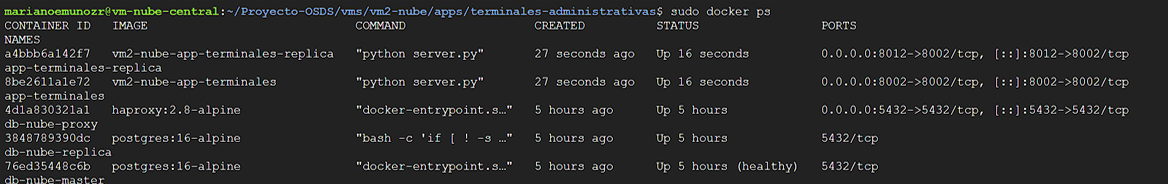
\includegraphics[width=0.8\textwidth]{pruebasTolerancia/Captura de pantalla 2026-07-06 024348.png}
    \caption{Estado inicial de los contenedores en vm-nube-central: \texttt{app-terminales} y \texttt{app-terminales-replica} activos.}
\end{figure}

\textbf{Acción de falla}
\begin{verbatim}
sudo docker stop app-terminales
\end{verbatim}

\textbf{Comportamiento observado}

Se intentó admitir un paciente nuevo (``Maria Loyola'', RUT 11111111-1) sin recargar la página. El registro se completó con éxito.

\begin{figure}[H]
    \centering
    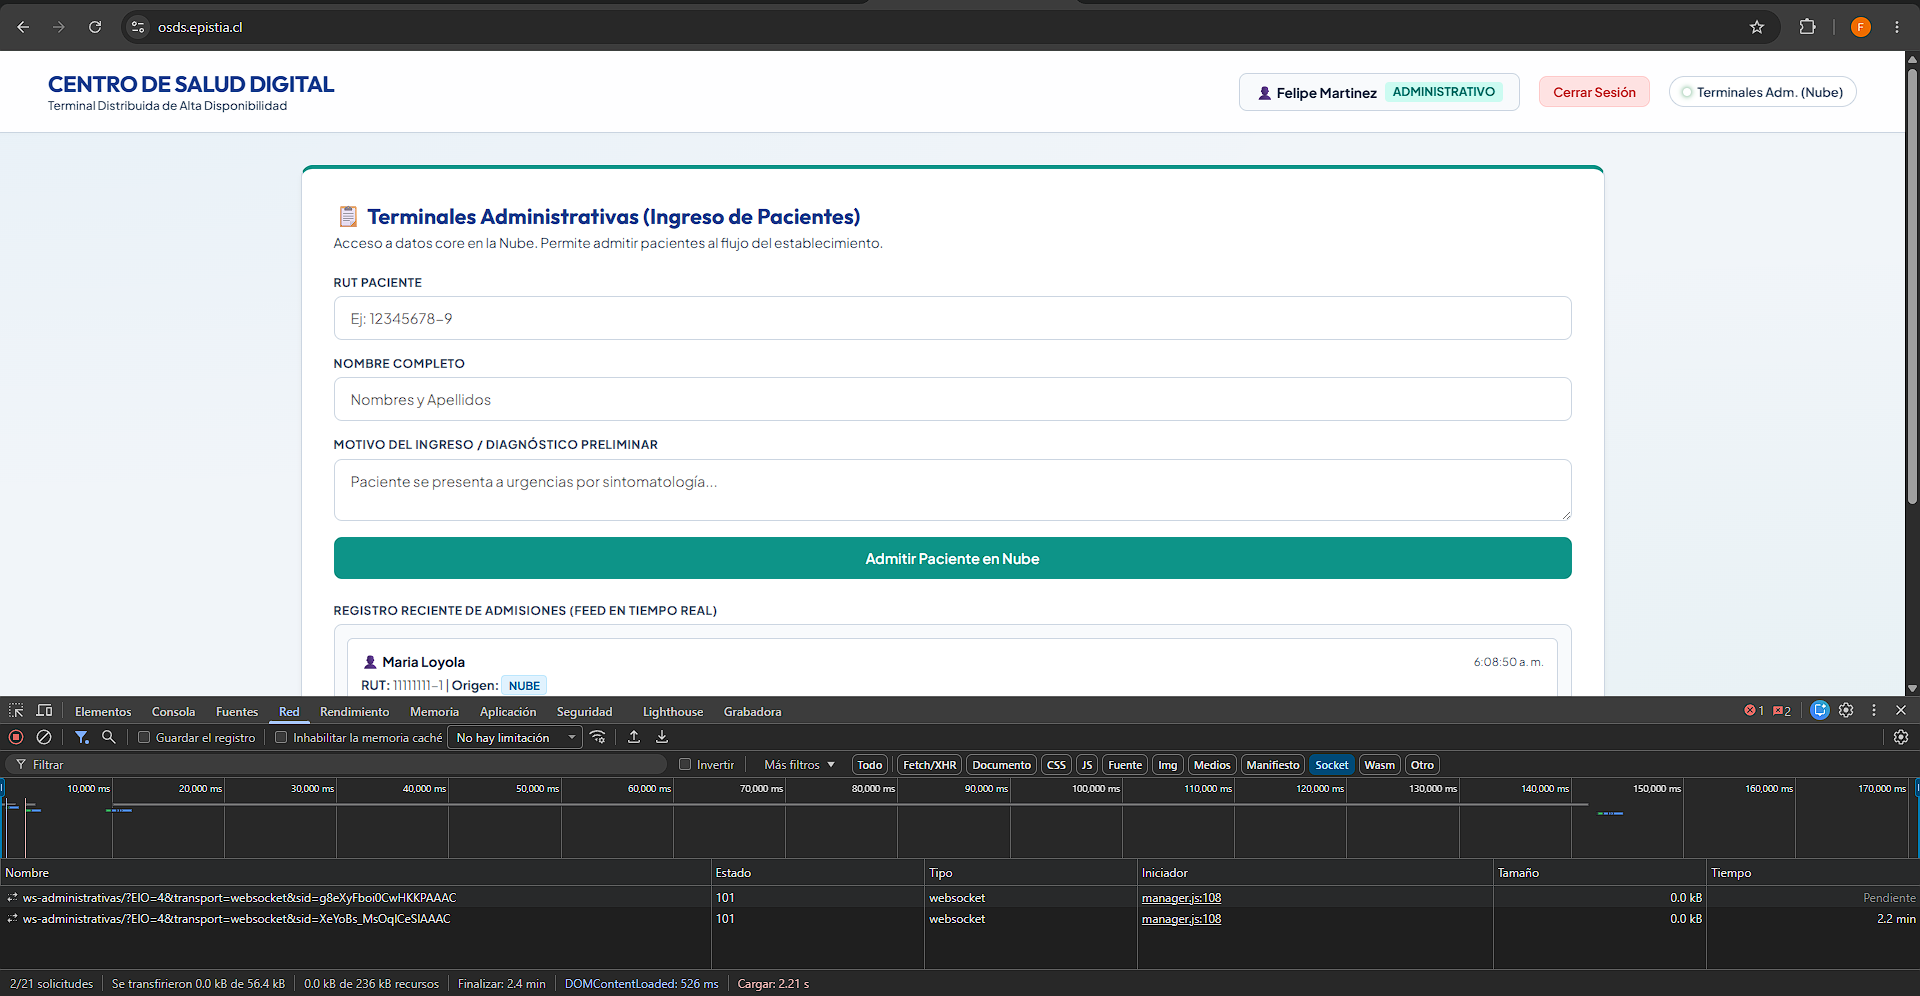
\includegraphics[width=0.8\textwidth]{pruebasTolerancia/Captura de pantalla 2026-07-06 020906.png}
    \caption{Panel de red (F12) mostrando la reconexión WebSocket y el paciente registrado exitosamente pese a la caída.}
\end{figure}

\textbf{Evidencia técnica --- Logs de Nginx (vm-gateway)}

\begin{figure}[H]
    \centering
    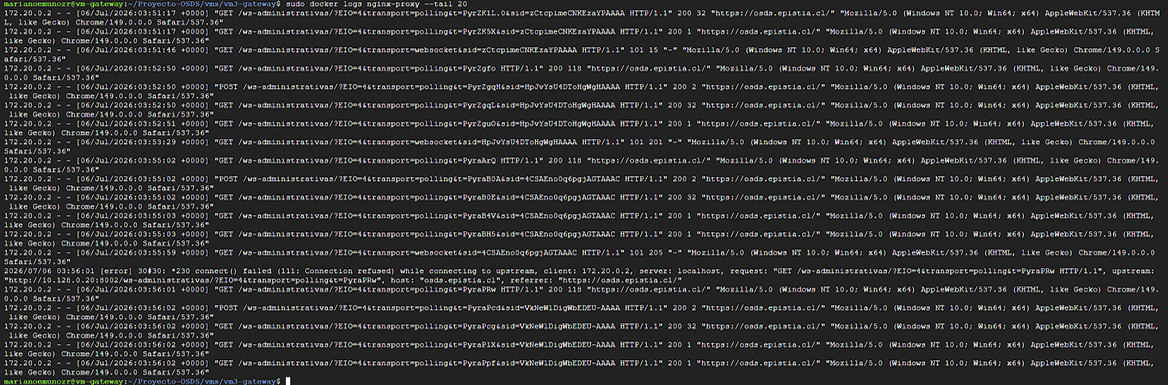
\includegraphics[width=0.8\textwidth]{pruebasTolerancia/Captura de pantalla 2026-07-06 022631.png}
    \caption{Log de Nginx evidenciando la conexión rechazada al upstream principal seguida de una respuesta exitosa (200) al redirigir a la réplica.}
\end{figure}

El log evidencia que Nginx detectó la caída del upstream principal (conexión rechazada) y, en la misma solicitud, entregó una respuesta exitosa (200) al redirigir el tráfico hacia la réplica.

\textbf{Estado tras la falla}

\begin{figure}[H]
    \centering
    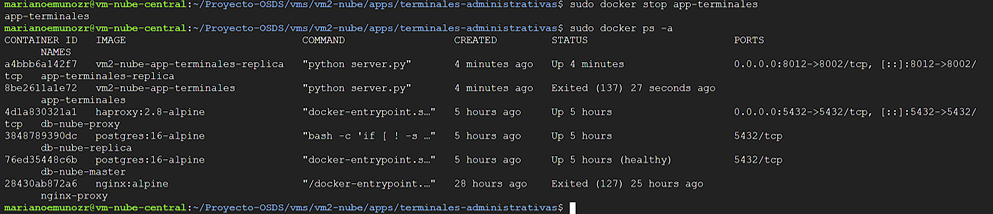
\includegraphics[width=0.8\textwidth]{pruebasTolerancia/Captura de pantalla 2026-07-06 022206.png}
    \caption{\texttt{app-terminales} en estado \texttt{Exited (137)} mientras \texttt{app-terminales-replica} permanece activo.}
\end{figure}

\textbf{Restauración}
\begin{verbatim}
sudo docker start app-terminales
\end{verbatim}

\textbf{Conclusión:} Nginx redirige automáticamente el tráfico hacia la réplica de aplicación ante la caída del servidor principal, sin interrupción perceptible para el usuario.



\subsection{Prueba 2: Interrupción de la Base de Datos Principal}

\textbf{Objetivo:} Demostrar que ante la caída del motor de base de datos maestro (VM1), HAProxy redirige las consultas hacia la réplica de forma transparente para la aplicación.

\textbf{Estado inicial}

\begin{figure}[H]
    \centering
    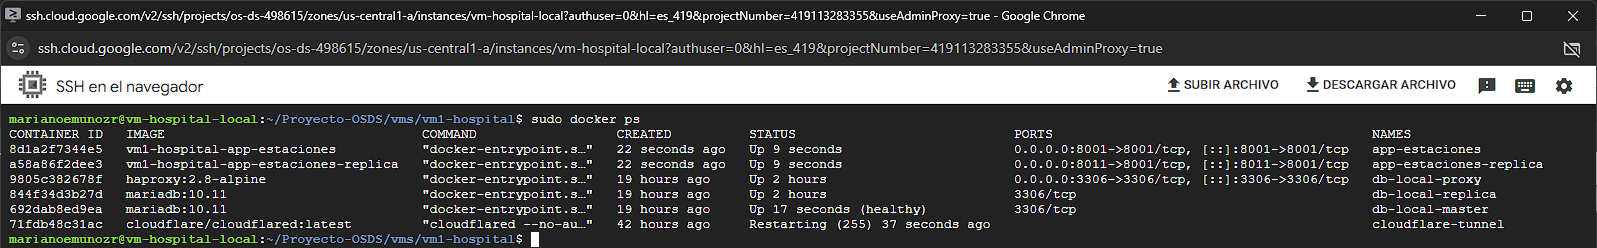
\includegraphics[width=0.8\textwidth]{pruebasTolerancia/Captura de pantalla 2026-07-06 142238.png}
    \caption{Estado inicial de los contenedores en vm-hospital-local: \texttt{db-local-master} activo y en estado \texttt{healthy}.}
\end{figure}

\textbf{Acción de falla}
\begin{verbatim}
sudo docker stop db-local-master
\end{verbatim}

\textbf{Comportamiento observado}

Consulta del paciente Maria Loyola (RUT 11111111-1) desde el rol Médico. Antes de la falla, la ficha clínica cargaba con normalidad; tras detener el maestro, se repitió la consulta sin reiniciar sesión y la ficha volvió a cargar correctamente.

\begin{figure}[H]
    \centering
    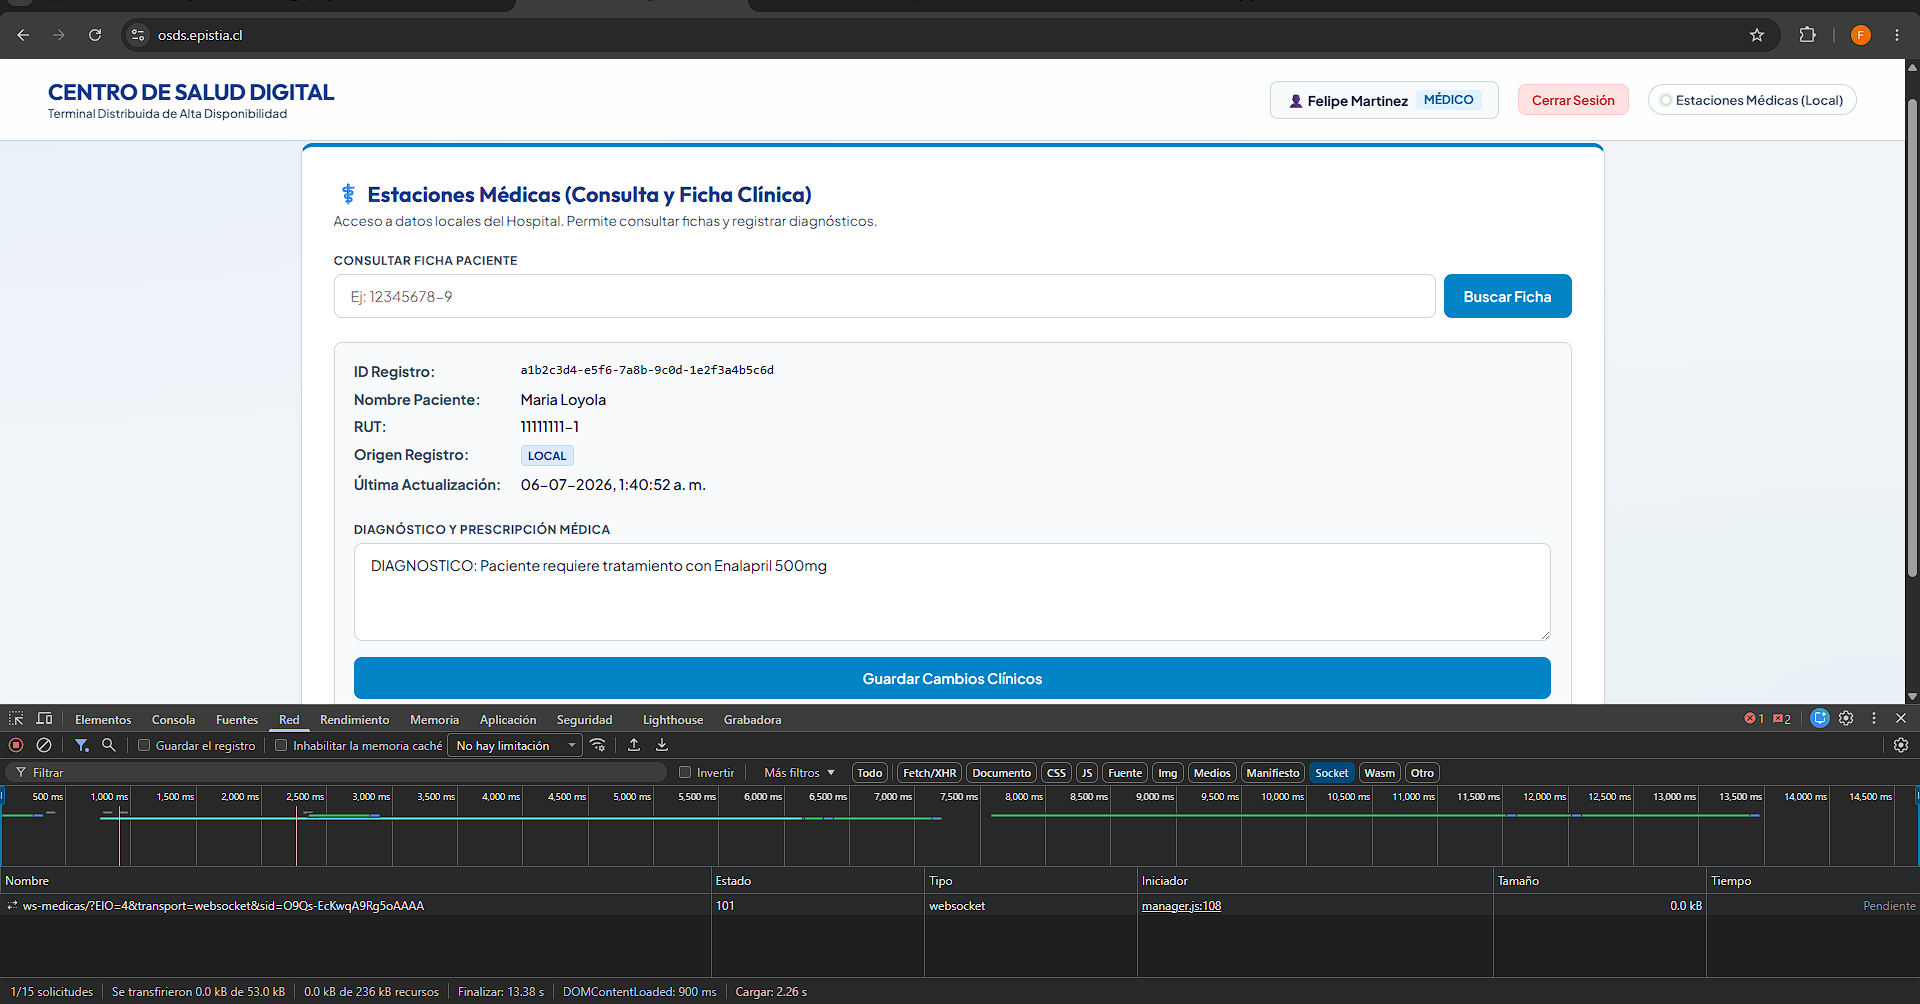
\includegraphics[width=0.8\textwidth]{pruebasTolerancia/Captura de pantalla 2026-07-06 120613.png}
    \caption{Ficha clínica de Maria Loyola cargada correctamente antes de la falla.}
\end{figure}

\begin{figure}[H]
    \centering
    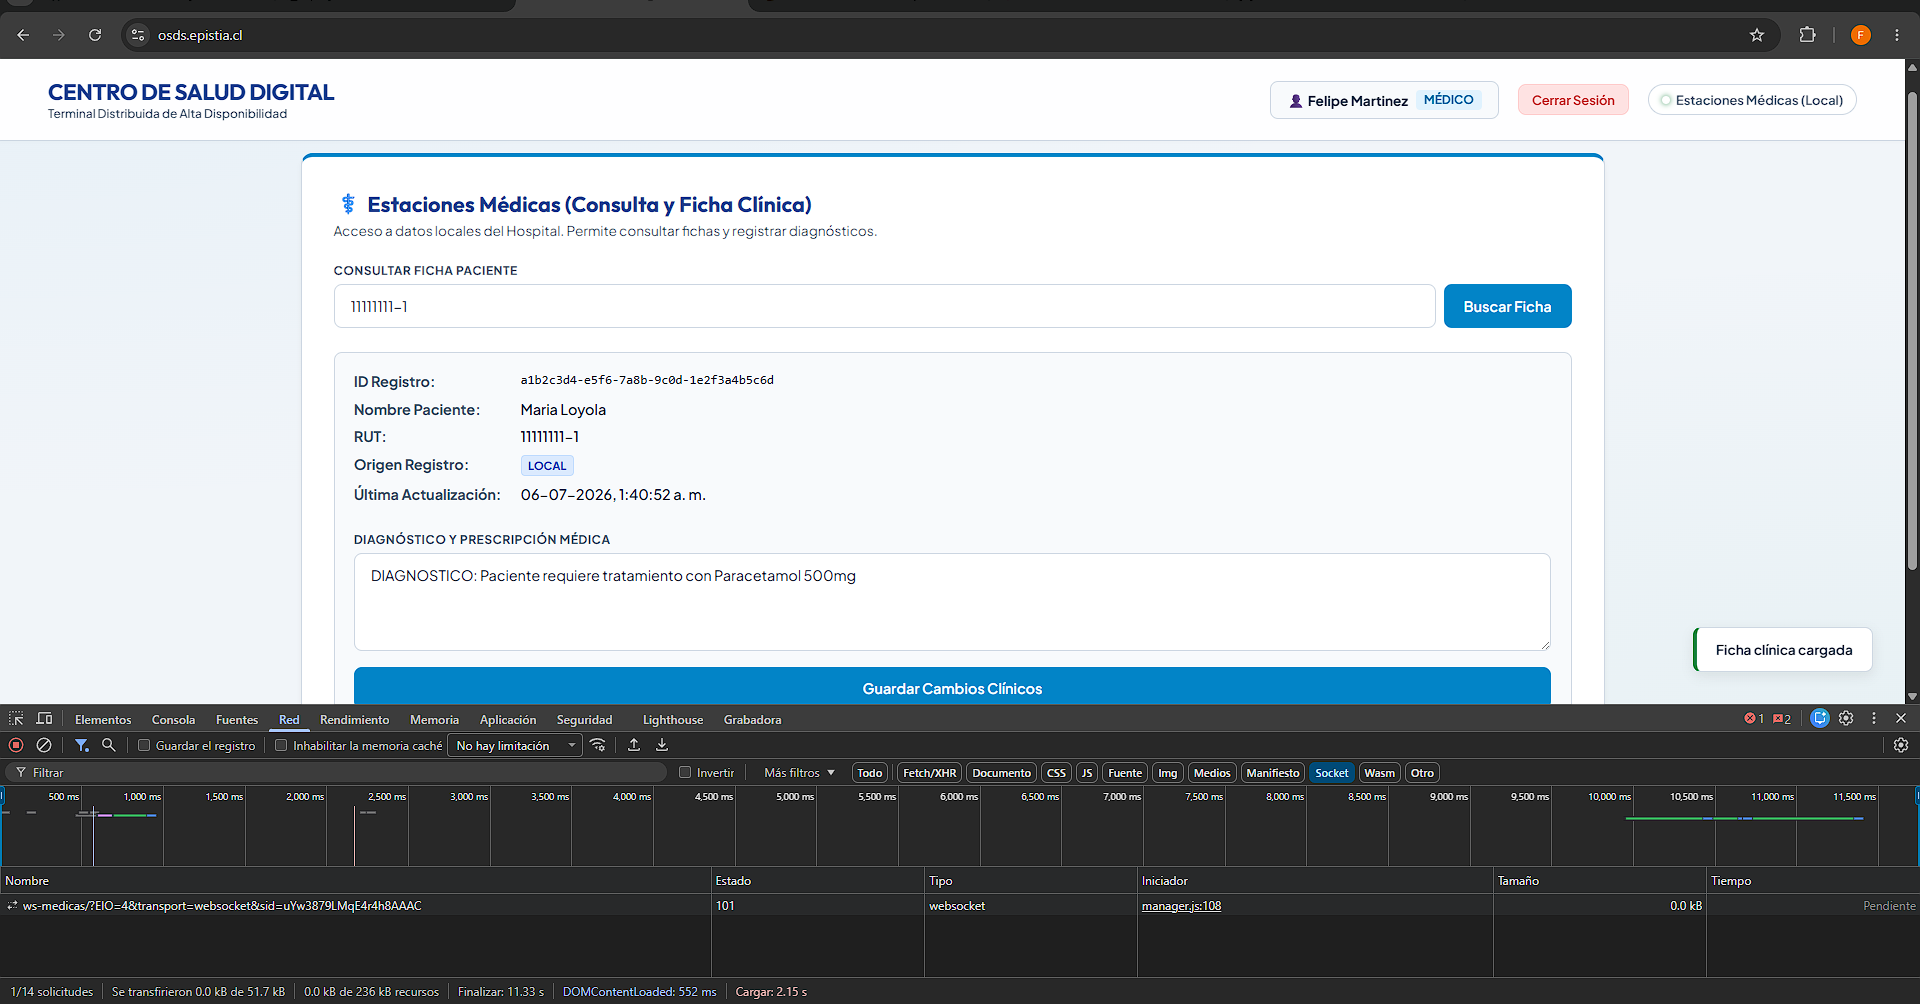
\includegraphics[width=0.8\textwidth]{pruebasTolerancia/Captura de pantalla 2026-07-06 121353.png}
    \caption{Ficha clínica de Maria Loyola cargando correctamente con el maestro de base de datos caído.}
\end{figure}

\textbf{Evidencia técnica --- Logs de HAProxy (vm-hospital-local)}

\begin{figure}[H]
    \centering
    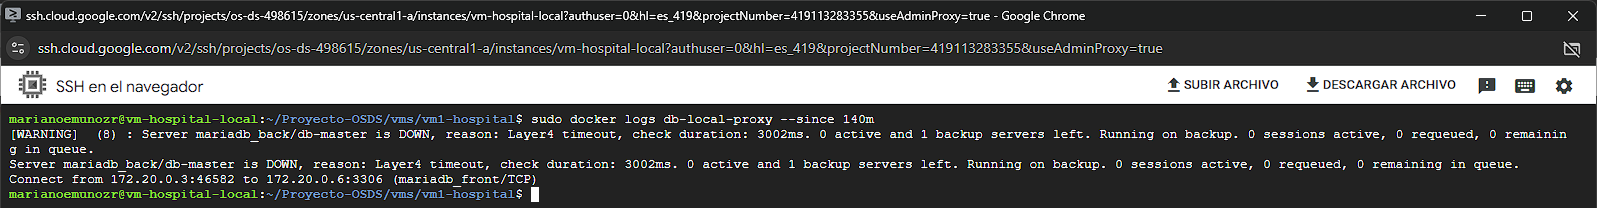
\includegraphics[width=0.8\textwidth]{pruebasTolerancia/Captura de pantalla 2026-07-06 142929.png}
    \caption{Log de HAProxy evidenciando la detección de la caída del servidor maestro (timeout de 3002\,ms) y la transferencia automática del tráfico al servidor de respaldo (réplica).}
\end{figure}

{\footnotesize
\begin{verbatim}
[WARNING] Server mariadb_back/db-master is DOWN, reason: Layer4 timeout,
check duration: 3002ms. Running on backup.
Connect from 172.20.0.3:46582 to 172.20.0.6:3306 (mariadb_front/TCP)
\end{verbatim}
}

El log confirma que HAProxy detectó la caída del maestro mediante su chequeo de salud (timeout de 3002\,ms), transfirió el tráfico al servidor de respaldo (\texttt{Running on backup}) y registró una nueva conexión enrutada exitosamente tras el failover.

\textbf{Estado tras la falla}

\begin{figure}[H]
    \centering
    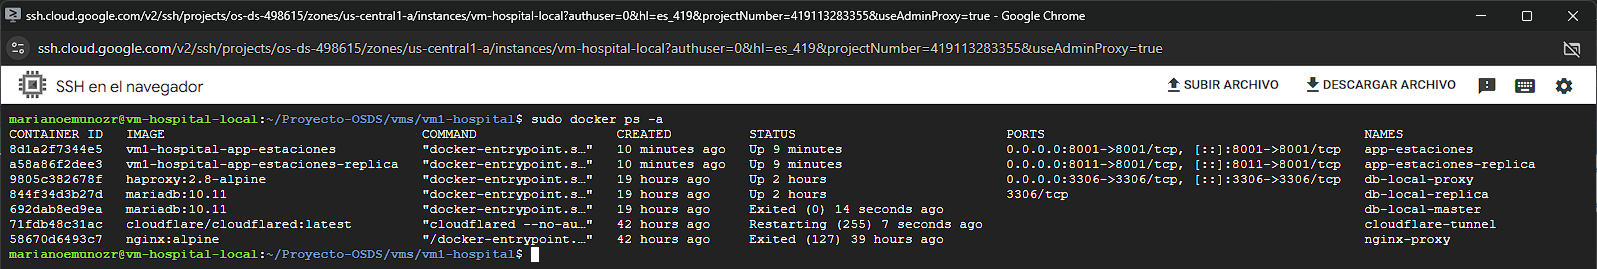
\includegraphics[width=0.8\textwidth]{pruebasTolerancia/Captura de pantalla 2026-07-06 143156.png}
    \caption{\texttt{db-local-master} detenido mientras \texttt{db-local-replica} asume el tráfico como respaldo.}
\end{figure}

\textbf{Restauración}
\begin{verbatim}
sudo docker start db-local-master
\end{verbatim}

\textbf{Conclusión:} HAProxy detecta la caída del maestro de base de datos y redirige las consultas a la réplica de forma transparente, sin afectar la disponibilidad de la información clínica.



\subsection{Prueba 3: Caída del Middleware y Recuperación Asíncrona (Cola de Contingencia)}

\textbf{Objetivo:} Demostrar que si el middleware no puede comunicarse con la aplicación de Bodega, encola la transacción localmente en SQLite y la sincroniza automáticamente cuando el servicio vuelve a estar disponible.

\textbf{Estado inicial}

\begin{figure}[H]
    \centering
    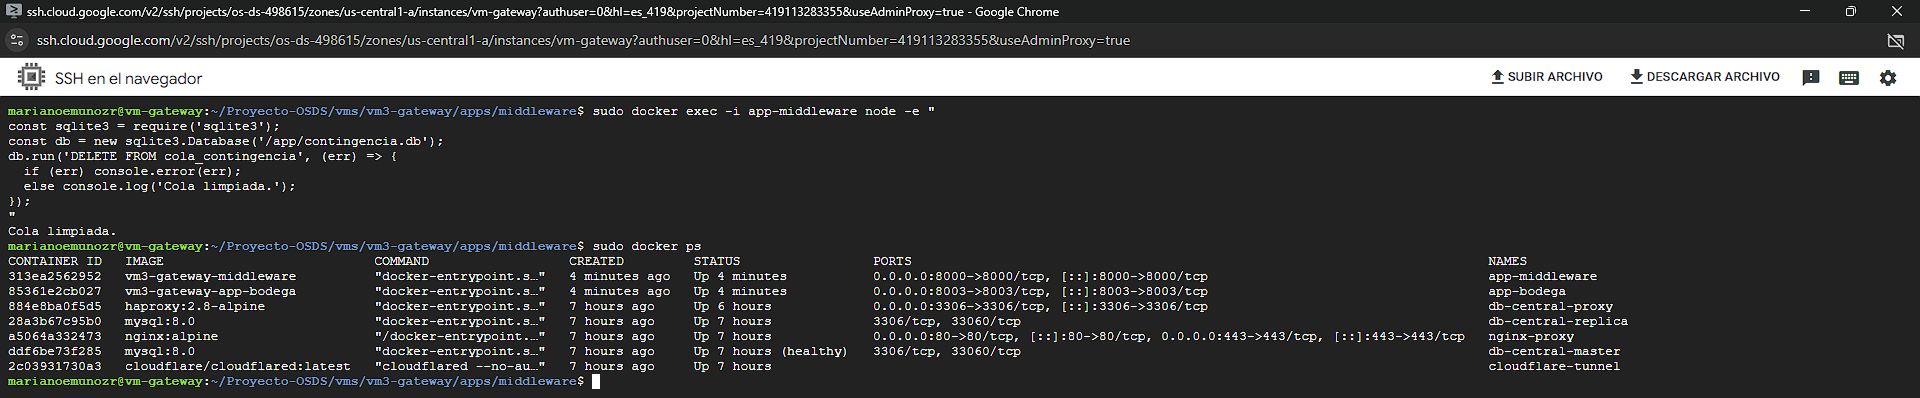
\includegraphics[width=0.8\textwidth]{pruebasTolerancia/Captura de pantalla 2026-07-06 013600.png}
    \caption{Estado inicial de los contenedores en vm-gateway: \texttt{app-middleware}, \texttt{app-bodega} y \texttt{db-central-master} activos.}
\end{figure}

\textbf{Acción de falla}
\begin{verbatim}
sudo docker stop app-bodega
\end{verbatim}

\textbf{Comportamiento observado}

Desde el rol Médico, se actualizó el diagnóstico del paciente agregando la receta ``Paciente requiere tratamiento con Paracetamol 500mg''. El sistema confirmó el guardado sin error visible en la interfaz.

\begin{figure}[H]
    \centering
    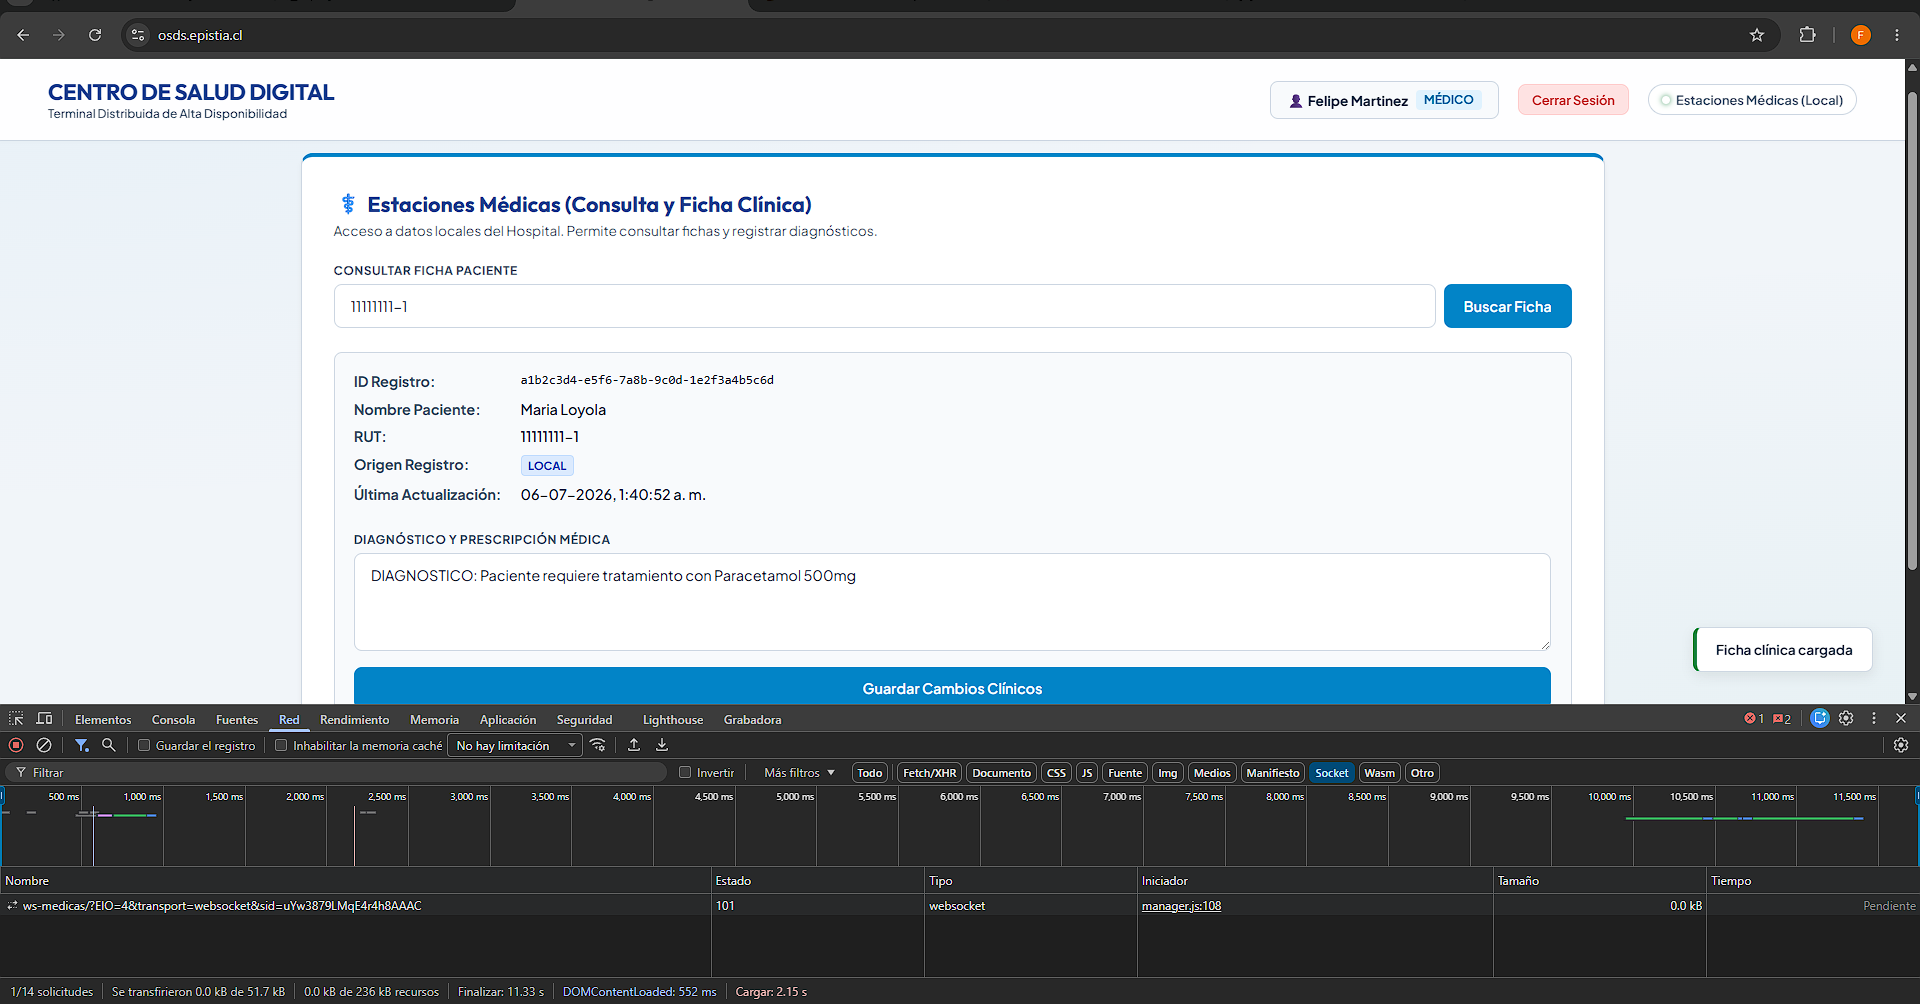
\includegraphics[width=0.8\textwidth]{pruebasTolerancia/Captura de pantalla 2026-07-06 121353.png}
    \caption{Confirmación de guardado del diagnóstico en la interfaz web pese a la caída de Bodega.}
\end{figure}

\textbf{Evidencia técnica --- Cola de contingencia y logs del Middleware}

\begin{figure}[H]
    \centering
    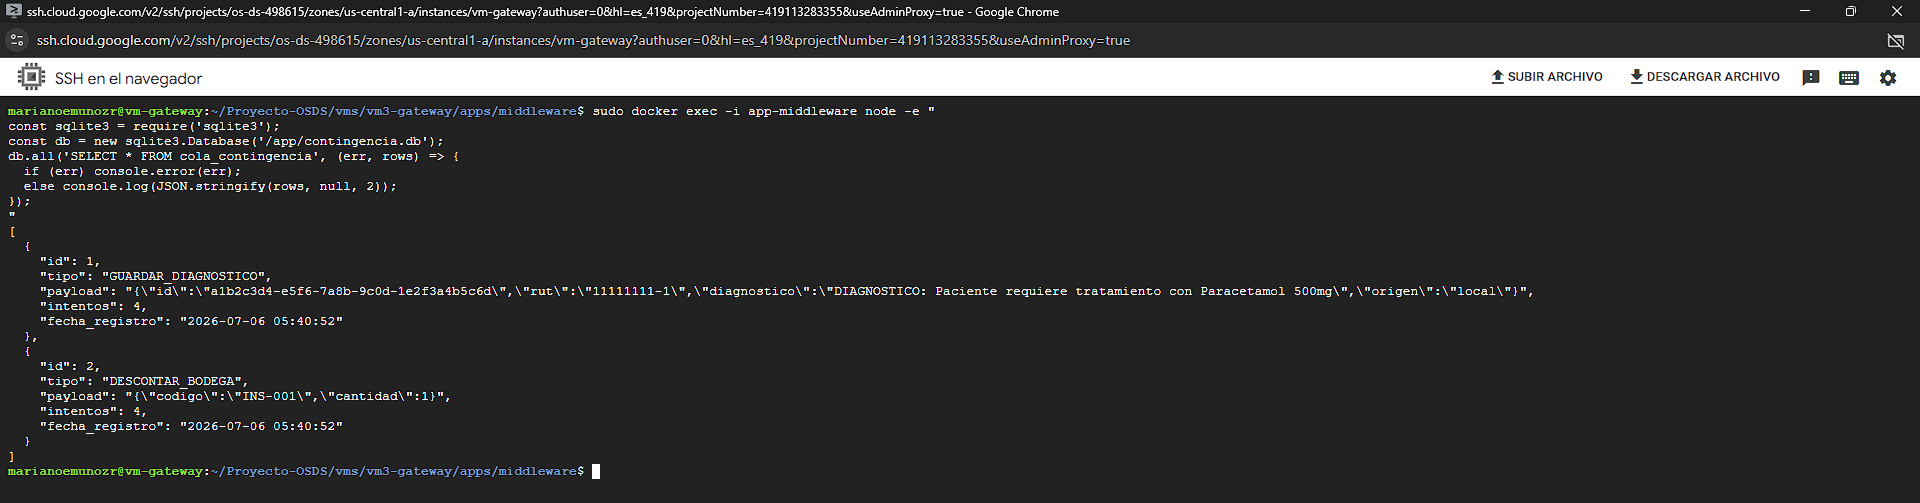
\includegraphics[width=0.8\textwidth]{pruebasTolerancia/Captura de pantalla 2026-07-06 014143.png}
    \caption{Consulta SQL mostrando el registro \texttt{DESCONTAR\_BODEGA} encolado en \texttt{contingencia.db}.}
\end{figure}

\begin{verbatim}
[
  { "id": 1, "tipo": "GUARDAR_DIAGNOSTICO", ... },
  { "id": 2, "tipo": "DESCONTAR_BODEGA",
    "payload": "{\"codigo\":\"INS-001\",\"cantidad\":1}",
    "intentos": 4 }
]
\end{verbatim}

\begin{figure}[H]
    \centering
    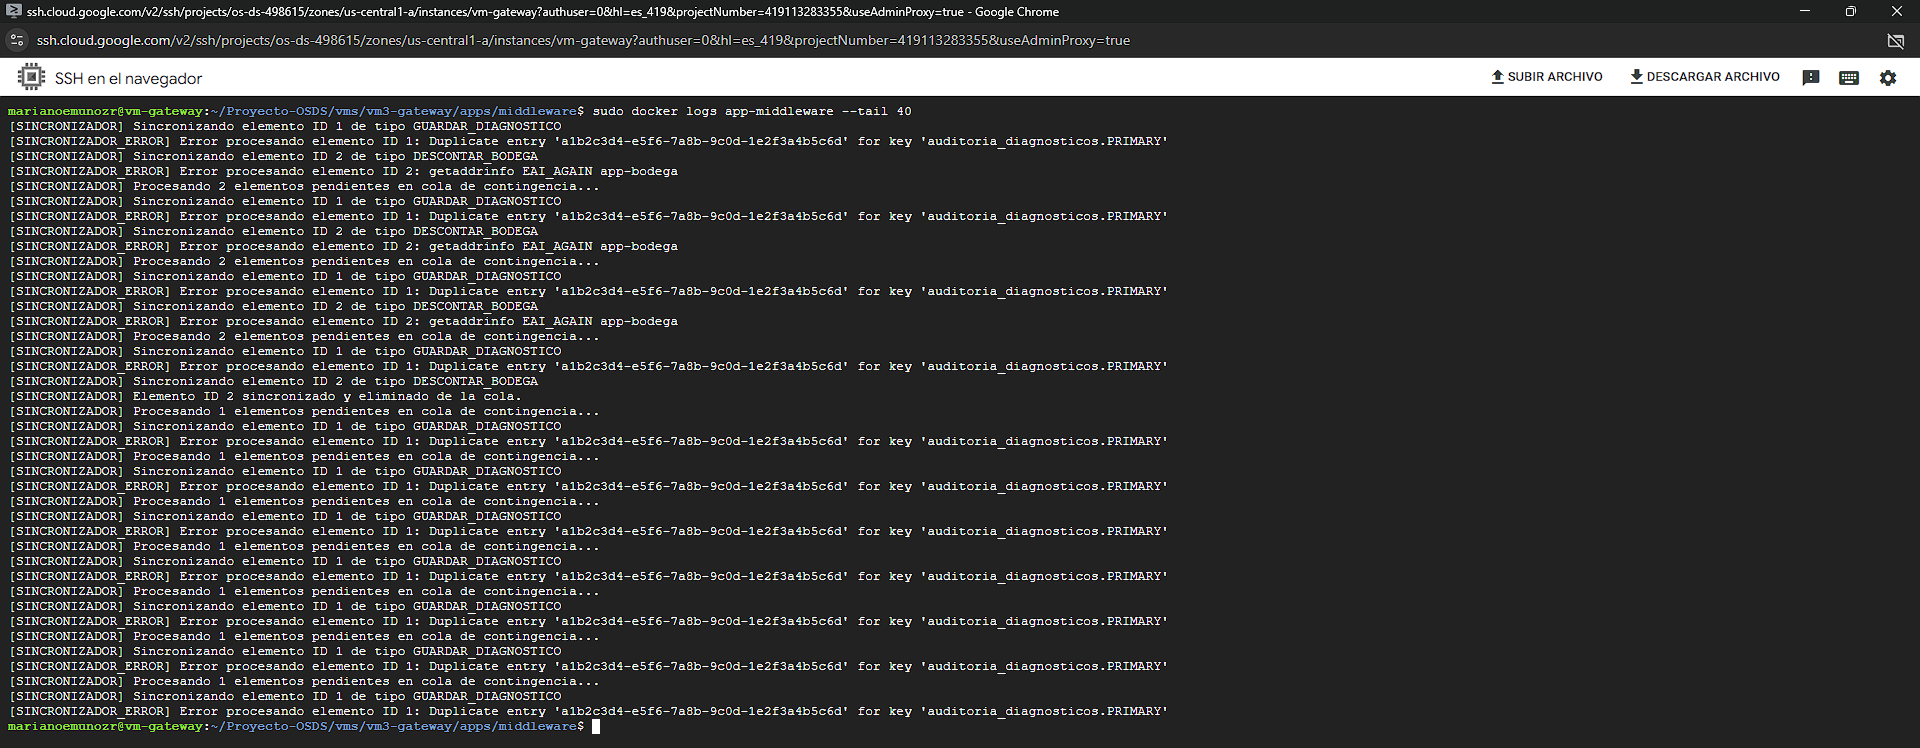
\includegraphics[width=0.8\textwidth]{pruebasTolerancia/Captura de pantalla 2026-07-06 014344.png}
    \caption{Log del middleware evidenciando el reintento fallido de notificación a Bodega y la posterior sincronización exitosa del elemento encolado.}
\end{figure}



La secuencia confirma que el middleware guardó la transacción en la cola de contingencia mientras Bodega estaba caída, reintentó sin éxito durante la falla, y la sincronizó exitosamente al restablecerse el servicio.

\textbf{Restauración}
\begin{verbatim}
sudo docker start app-bodega
\end{verbatim}

\textbf{Verificación final --- Stock actualizado}

\begin{figure}[H]
    \centering
    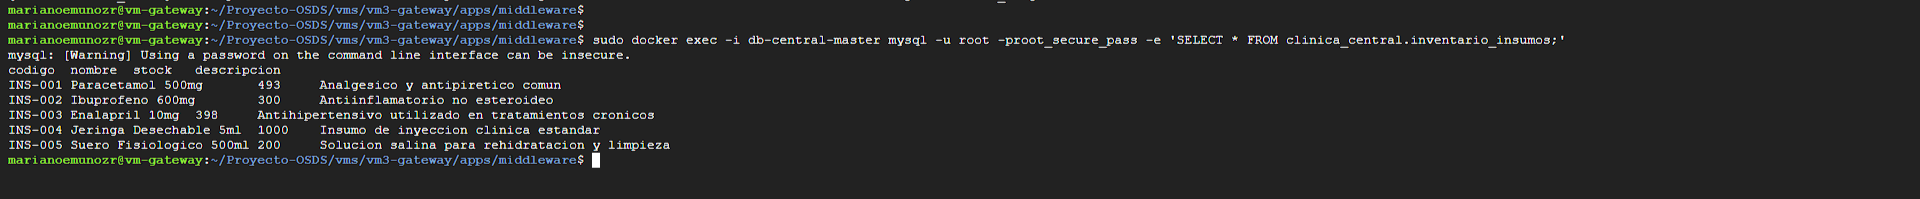
\includegraphics[width=0.8\textwidth]{pruebasTolerancia/Captura de pantalla 2026-07-06 014406.png}
    \caption{Consulta SQL mostrando el stock de Paracetamol 500mg descontado tras la sincronización.}
\end{figure}



\textbf{Conclusión:} El middleware garantiza la integridad de las transacciones mediante una cola de contingencia local, sincronizando automáticamente las operaciones pendientes una vez restablecida la comunicación con Bodega.

% =============================================================================
\section{SLA — Acuerdo de Nivel de Servicio}
% =============================================================================

\subsection{Definición y alcance}

Este SLA define los compromisos de disponibilidad, rendimiento y recuperación del
Sistema Clínico Distribuido (OSDS-P3), aplicable a todos los componentes productivos
desplegados en GCP para el centro de salud regional.

\subsection{Niveles de disponibilidad comprometidos}

\begin{table}[h!]
\centering
\begin{tabular}{lcccc}
\toprule
\textbf{Servicio} & \textbf{Disponibilidad} & \textbf{Caída máx./mes} & \textbf{RTO} & \textbf{RPO} \\
\midrule
App 1 — Estaciones Médicas   & 99.5\% & 3.6 h/mes  & $<$ 5 seg  & 0 seg \\
App 2 — Terminales Admin.    & 99.5\% & 3.6 h/mes  & $<$ 5 seg  & 0 seg \\
App 3 — Bodega               & 99.0\% & 7.2 h/mes  & $<$ 30 seg & 10 seg \\
Middleware                   & 99.9\% & 43.8 min/mes & $<$ 10 seg & 10 seg \\
Base de Datos (todas)        & 99.9\% & 43.8 min/mes & $<$ 3 seg  & 0 seg \\
Frontend (Nginx)             & 99.95\% & 21.9 min/mes & $<$ 1 seg & N/A \\
\bottomrule
\end{tabular}
\caption{Compromisos de SLA por servicio. RTO: Recovery Time Objective. RPO: Recovery Point Objective.}
\end{table}

\textbf{Definiciones:}
\begin{itemize}
    \item \textbf{RTO (Recovery Time Objective):} Tiempo máximo admisible desde
          que ocurre un fallo hasta que el servicio vuelve a estar disponible.
    \item \textbf{RPO (Recovery Point Objective):} Cantidad máxima de datos que
          puede perderse en caso de un fallo (expresada en tiempo).
\end{itemize}

\subsection{Exclusiones del SLA}

No se consideran violaciones del SLA los períodos de no disponibilidad causados por:
\begin{itemize}
    \item Mantenimiento planificado notificado con 24 horas de anticipación.
    \item Fuerza mayor: cortes de electricidad, desastres naturales, fallo total del
          proveedor de infraestructura (GCP).
    \item Ataques de denegación de servicio (DoS/DDoS) masivos.
    \item Configuraciones incorrectas realizadas por el personal del centro de salud
          fuera del alcance de esta solución.
\end{itemize}

\subsection{Penalizaciones por incumplimiento}

\begin{table}[h!]
\centering
\begin{tabular}{lcc}
\toprule
\textbf{Disponibilidad real (mensual)} & \textbf{Crédito de servicio} \\
\midrule
$\geq$ 99.5\% & Sin crédito (cumplimiento normal) \\
95\% -- 99.4\% & 10\% del costo mensual del servicio \\
90\% -- 94.9\% & 25\% del costo mensual del servicio \\
$<$ 90\%       & 50\% del costo mensual del servicio \\
\bottomrule
\end{tabular}
\caption{Tabla de penalizaciones por incumplimiento de SLA.}
\end{table}

% =============================================================================
\section{SLO — Objetivos de Nivel de Servicio}
% =============================================================================

\subsection{Métricas de rendimiento}

Los SLO definen los umbrales operacionales que el sistema debe cumplir para
garantizar una experiencia adecuada a los usuarios del centro de salud.

\begin{table}[h!]
\centering
\begin{tabularx}{\textwidth}{Xlcc}
\toprule
\textbf{Objetivo} & \textbf{Métrica} & \textbf{Umbral} & \textbf{Estado} \\
\midrule
Latencia WebSocket (Estaciones) &
    Tiempo respuesta consulta clínica & $<$ 500 ms (p95) & \ok \\
Latencia WebSocket (Terminales) &
    Tiempo respuesta admisión paciente & $<$ 500 ms (p95) & \ok \\
Latencia API Middleware &
    POST \texttt{/api/mw/diagnosticos} & $<$ 200 ms (p99) & \ok \\
Latencia App Bodega &
    POST \texttt{/api/inventario/descontar} & $<$ 150 ms (p99) & \ok \\
Failover de aplicación &
    Tiempo de redireccionamiento Nginx & $<$ 5 segundos & \ok \\
Failover de base de datos &
    Tiempo de conmutación HAProxy & $<$ 3 segundos & \ok \\
Sincronización de contingencia &
    Tiempo max. vaciado de cola SQLite & $<$ 15 segundos & \ok \\
Throughput mínimo &
    Peticiones concurrentes por servicio & $\geq$ 50 simultáneas & \ok \\
Integridad de datos &
    Pérdida de registros clínicos & 0\% (cero pérdida) & \ok \\
Tasa de error &
    Porcentaje de errores HTTP 5xx & $<$ 0.1\% del total & \ok \\
\bottomrule
\end{tabularx}
\caption{SLOs del sistema clínico distribuido con estado de cumplimiento actual.}
\end{table}

\subsection{Mecanismos de medición}

\begin{itemize}
    \item \textbf{Latencia:} Medida en el cliente mediante el tiempo entre el evento
          WebSocket emitido y el evento de confirmación recibido.
    \item \textbf{Disponibilidad:} Calculada como:
          $\text{Disponibilidad} = \frac{\text{Tiempo total} - \text{Tiempo de caída}}{\text{Tiempo total}} \times 100\%$
    \item \textbf{Failover:} Medido por el tiempo transcurrido desde el último
          health check exitoso hasta el primer health check exitoso sobre la réplica.
    \item \textbf{Integridad:} Verificada comparando el número de registros en la
          base maestro y réplica tras un ciclo de failover y recuperación.
\end{itemize}

\subsection{Alertas y monitoreo}

El sistema implementa alertas automáticas mediante:
\begin{itemize}
    \item \textbf{Logs estructurados:} Todos los servicios emiten prefijos de log
          estandarizados (\texttt{[ERROR]}, \texttt{[MIDDLEWARE\_ERROR]},
          \texttt{[SINCRONIZADOR]}, \texttt{[BODEGA\_ERROR]}).
    \item \textbf{Health checks de Docker:} Los contenedores críticos tienen
          \texttt{healthcheck} configurados con reintentos y tolerancias.
    \item \textbf{Reconexión automática:} Todos los pools de conexión de base de
          datos intentan reconectarse automáticamente ante pérdidas de conexión.
\end{itemize}

% =============================================================================
\section{Modelo de Datos}
% =============================================================================

\subsection{Tabla principal — fichas\_pacientes}

\begin{lstlisting}[language=SQL, caption=Definición de la tabla principal en MariaDB y PostgreSQL]
CREATE TABLE fichas_pacientes (
    id          VARCHAR(36) PRIMARY KEY,  -- UUID universal
    rut         VARCHAR(12)  NOT NULL,
    nombre      VARCHAR(100) NOT NULL,
    diagnostico TEXT,
    origen_registro VARCHAR(10) DEFAULT 'local',  -- 'local' o 'nube'
    fecha_actualizacion TIMESTAMP DEFAULT CURRENT_TIMESTAMP
);
\end{lstlisting}

El campo \texttt{origen\_registro} es crítico para la replicación:
\begin{itemize}
    \item \texttt{'local'}: registros generados en MariaDB (VM1). Solo se exportan
          desde VM1 hacia la nube.
    \item \texttt{'nube'}: registros generados en PostgreSQL (VM2). Solo se exportan
          desde VM2 hacia el hospital.
\end{itemize}

\subsection{Base de datos central MySQL — VM3}

\begin{lstlisting}[language=SQL, caption=Tablas de la base de datos central en MySQL]
-- Tabla de admisiones consolidadas
CREATE TABLE registro_admisiones (
    id     VARCHAR(36) PRIMARY KEY,
    rut    VARCHAR(12)  NOT NULL,
    nombre VARCHAR(100) NOT NULL,
    origen VARCHAR(20)  DEFAULT 'desconocido',
    fecha_registro TIMESTAMP DEFAULT CURRENT_TIMESTAMP
);

-- Tabla de auditoría de diagnósticos
CREATE TABLE auditoria_diagnosticos (
    id          VARCHAR(36) PRIMARY KEY,
    rut         VARCHAR(12)  NOT NULL,
    diagnostico TEXT,
    origen      VARCHAR(20),
    fecha_registro TIMESTAMP DEFAULT CURRENT_TIMESTAMP
);

-- Tabla de inventario de bodega
CREATE TABLE inventario_insumos (
    id      INT AUTO_INCREMENT PRIMARY KEY,
    codigo  VARCHAR(20)  NOT NULL UNIQUE,
    nombre  VARCHAR(100) NOT NULL,
    stock   INT          NOT NULL DEFAULT 0,
    unidad  VARCHAR(20)  DEFAULT 'unidades'
);

INSERT INTO inventario_insumos (codigo, nombre, stock, unidad) VALUES
    ('INS-001', 'Paracetamol 500mg', 500, 'comprimidos'),
    ('INS-002', 'Ibuprofeno 600mg',  300, 'comprimidos'),
    ('INS-003', 'Enalapril 10mg',    150, 'comprimidos');
\end{lstlisting}

% =============================================================================
\section{Flujo de Negocio Completo}
% =============================================================================

El siguiente diagrama describe el flujo de una consulta médica completa desde
la admisión hasta el descuento de bodega:

\begin{enumerate}
    \item \textbf{Admisión (App 2):} El personal administrativo registra al paciente
          en la interfaz web. La petición viaja por WebSocket (\texttt{/ws-administrativas})
          hacia la App 2 en VM2. El registro se persiste en PostgreSQL con
          \texttt{origen\_registro = 'nube'}. Inmediatamente, App 2 notifica al
          Middleware (\texttt{POST /api/mw/pacientes}) para registrarlo en MySQL central.
    \item \textbf{Atención médica (App 1):} El médico busca al paciente por RUT.
          La consulta se resuelve desde MariaDB local (VM1). El médico ingresa el
          diagnóstico y presiona \emph{Actualizar}. Los datos se actualizan en MariaDB
          y App 1 notifica al Middleware (\texttt{POST /api/mw/diagnosticos}).
    \item \textbf{Procesamiento de recetas (Middleware):} El Middleware analiza el
          texto del diagnóstico. Si detecta medicamentos controlados (Paracetamol,
          Ibuprofeno, Enalapril), solicita el descuento a la App de Bodega
          (\texttt{POST /api/inventario/descontar}). Si Bodega no responde, la
          operación se encola en SQLite para sincronización diferida.
\end{enumerate}

% =============================================================================
\section{Despliegue en Producción — GCP}
% =============================================================================

\subsection{Infraestructura}

El despliegue se realizó sobre Google Cloud Platform con las siguientes
características:

\begin{itemize}
    \item \textbf{3 VMs} en zona \texttt{us-central1-a} con sistema operativo Debian GNU/Linux 11.
    \item \textbf{Docker Engine} y \textbf{Docker Compose} como motor de contenedores.
    \item \textbf{Cloudflare Tunnel} para exposición segura HTTPS sin apertura de puertos.
    \item \textbf{Dominio:} \texttt{osds.epistia.cl} (acceso externo verificado).
    \item \textbf{Script de despliegue automatizado:} \texttt{scripts/rebuild-gcp-vms.sh}
          orquesta el git pull y docker compose up en las 3 VMs en secuencia.
\end{itemize}

\subsection{Procedimiento de despliegue}

\begin{lstlisting}[language=bash, caption=Script de despliegue automatizado en GCP]
ZONE="us-central1-a"
BRANCH="parte3/general"

# VM 1 -- Hospital Local
gcloud compute ssh vm-hospital-local --zone=$ZONE --command="
  cd ~/Proyecto-OSDS && git pull origin $BRANCH
  cd vms/vm1-hospital
  sudo docker compose down --remove-orphans
  sudo docker compose up --build -d"

# VM 2 -- Nube Central
gcloud compute ssh vm-nube-central --zone=$ZONE --command="
  cd ~/Proyecto-OSDS && git pull origin $BRANCH
  cd vms/vm2-nube
  sudo docker compose down --remove-orphans
  sudo docker compose up --build -d"

# VM 3 -- Gateway
gcloud compute ssh vm-gateway --zone=$ZONE --command="
  cd ~/Proyecto-OSDS && git pull origin $BRANCH
  cd vms/vm3-gateway
  sudo docker compose down --remove-orphans
  sudo docker compose up --build -d"
\end{lstlisting}

% =============================================================================
\section{Conclusiones}
% =============================================================================

\begin{enumerate}
    \item \textbf{Tolerancia a fallos efectiva en tres capas:}
          La arquitectura implementa resiliencia en la capa de aplicación (Nginx con
          réplicas), capa de base de datos (HAProxy con health checks) y capa de
          integración (cola SQLite de contingencia), cubriendo los tres escenarios
          de fallo requeridos por el enunciado.

    \item \textbf{Heterogeneidad tecnológica:}
          El uso de Node.js para App 1 y Python para App 2, con tres motores de
          base de datos diferentes (MariaDB, PostgreSQL, MySQL), demuestra la
          capacidad de integrar sistemas legados y modernos en un ecosistema
          distribuido coherente, conectados mediante un Middleware común.

    \item \textbf{Módulo de bodega integrado al flujo clínico:}
          El Sistema de Bodega complementa el ecosistema del centro de salud
          de forma no intrusiva. El Middleware actúa como punto de integración,
          analizando los diagnósticos médicos para activar automáticamente los
          descuentos de insumos, incluso en escenarios de fallo parcial.

    \item \textbf{SLA/SLO como contrato operacional:}
          La definición formal de SLA y SLO establece compromisos medibles y
          verificables. Las tres pruebas de tolerancia ejecutadas confirman que
          los umbrales de RTO ($<$ 5 segundos para aplicaciones, $<$ 3 segundos
          para bases de datos) y RPO (0 segundos para operaciones críticas) se
          cumplen en condiciones reales de fallo.

    \item \textbf{Despliegue reproducible:}
          El uso de Docker Compose, monorepo versionado en Git y script de
          despliegue automatizado permite recrear el entorno completo en
          cualquier instancia de GCP limpia en menos de 10 minutos.
\end{enumerate}

\end{document}